\section{Problem statement and model}
\label{sec:Chapter_III}
\subsection{Problem statement}

An instance consists of $n$ jobs, $N_M$ robotic arms, and $N_A$ vehicles (AGVs) on a shop-floor graph (Table~\ref{tab:notation}).
Job $j$ is a fixed chain of $n_j$ operations $O_{j1}\to\cdots\to O_{jn_j}$; operation $O_{ji}$ may be processed on any arm in its option set $\Omega_{ji}\subseteq M$, taking an arm-dependent time $t^P_{jim}$.
Arms occupy fixed nodes, and the fleet moves jobs between them.
Four decision groups are solved at once:
(i)~assign each operation to an arm in $\Omega_{ji}$;
(ii)~sequence the operations on each arm;
(iii)~assign the induced transport tasks to vehicles and sequence each vehicle's tasks;
(iv)~plan for every move a path that is conflict-free in time and space, waiting allowed.
The objective is to minimize the makespan $C_{\max}$.

\begin{table}[t]
\caption{Notation.}
\label{tab:notation}
\footnotesize
\begin{tabular}{@{}ll@{}}
\toprule
Symbol & Meaning \\
\midrule
$J=\{1,\dots,n\}$, $O_{ji}$ & jobs; $i$-th operation of job $j$, $i\le n_j$ \\
$M=\{1,\dots,N_M\}$, $\Omega_{ji}\subseteq M$ & robotic arms; option set of $O_{ji}$ \\
$t^P_{jim}$ & processing time of $O_{ji}$ on arm $m\in\Omega_{ji}$ \\
$K=\{1,\dots,N_A\}$ & homogeneous unit-load vehicles \\
$G=(V,E)$, $\tau_e$ & shop-floor graph; traversal time of corridor $e$ \\
$v_0$, $\mathrm{loc}(m)$ & load/unload point; node of arm $m$ \\
$t^{*}(a,b)$ & shortest-path time $a\to b$ in $G$, ignoring contention \\
$\delta_{\mathrm{ret}}\in\{0,1\}$ & finished job returns to $v_0$ (baseline $1$) \\
$S_{ji}$, $C_{ji}$, $A_{ji}$, $C_{\max}$ & start, completion, material arrival; makespan \\
\bottomrule
\end{tabular}
\end{table}

\subsection{Modelling assumptions}
\label{sec:assumptions}

\begin{enumerate}[label=\textbf{A\arabic*.},leftmargin=*,topsep=2pt,itemsep=1pt]
\item \textbf{Static instance and complete information.} All $n$ jobs are at $v_0$ at $t=0$; no release or due dates. Processing data, $G$, and vehicle states are known at planning time.

\item \textbf{Jobs.} Fixed precedence chain per job. Processing and transport are non-preemptive; jobs cannot be split; no exogenous precedence among jobs.

\item \textbf{Robotic arms: partial flexibility and heterogeneous times.} $O_{ji}$ may run on any $m\in\Omega_{ji}$ (most operations have $|\Omega_{ji}|\ge 2$; $\Omega_{ji}=M$ is a special case). Times $t^P_{jim}$ vary with the arm and need not be proportional across arms. An arm processes one operation at a time and does not fail; sequence-dependent setup is folded into $t^P_{jim}$.

\item \textbf{Buffers and loading.} Ample input/output buffers and storage at $v_0$, so no blocking. Loading and unloading are negligible and do not occupy the arm.

\item \textbf{Vehicles.} $N_A$ homogeneous unit-load vehicles at constant speed, empty or loaded; no acceleration or battery. All stand empty and available at $v_0$ at $t=0$. A task is a one-way move---$v_0$ to the first arm, between successive distinct arms, or, when $\delta_{\mathrm{ret}}=1$, last arm back to $v_0$; any vehicle may take any task, so a job's moves may be relayed across vehicles. After unloading, a vehicle is not forced back to $v_0$; it follows its own task chain, and routing may postpone its departure.

\item \textbf{Road network and conflict-freedom.} $G$ is strongly connected; each $\tau_e$ is a known constant. Corridors are \emph{exclusive}: both directions of $e$ share one reservation, so at most one vehicle occupies $e$ at a time (no head-on conflict, no overtaking). Occupancy is half-open, $[t,\,t+\tau_e)$, so a second vehicle may enter at $t+\tau_e$. Nodes have ample berths, separate from the traversal resource; waits occur at berths and are always permitted.

\item \textbf{Out of scope.} Machine and vehicle failures, finite buffers and blocking, battery charging, and dynamic job arrivals~\cite{gui2023dynamic,xiong2024dynamic} are left to future work (item~(5) of Section~\ref{sec:future_work}).
\end{enumerate}

A1, A2, A4, and A5 are standard in FJSP\_PT~\cite{xin2025review}; our problem is defined by A3 and A6, which make transport duration an output of routing rather than a constant matrix entry.
Deadlock-freedom is not assumed: Proposition~\ref{prop:decodable} uses A4 and A6 to prove that any assignment and sequence decodes into a conflict-free, deadlock-free timetable, so the search need not repair infeasible solutions.

\subsection{Decision variables and induced transport tasks}

Let $x_{jim}\in\{0,1\}$ indicate that $O_{ji}$ is assigned to arm $m$; write $\mathrm{m}(j,i)$ for the chosen arm and $d_{ji}=\mathrm{loc}(\mathrm{m}(j,i))$ for its node.
When $\delta_{\mathrm{ret}}=1$, a zero-duration dummy operation $O_{j,n_j+1}$ at $v_0$ represents the return, so return moves share the task notation and the makespan is always the completion of each job's last operation.
Unlike in vehicle routing, transport tasks are not an input but are \emph{induced} by the assignment:
\begin{equation}
\label{eq:tasks}
\mathcal{T}(x)=\Bigl\{\,(j,i)\ :\ d_{j,i-1}\neq d_{ji}\,\Bigr\},
\qquad d_{j0}\equiv v_0 ,
\end{equation}
where task $(j,i)$ moves job $j$ from $d_{j,i-1}$ to $d_{ji}$ and is ready at $r_{ji}=C_{j,i-1}$ ($C_{j0}=0$).
Decision~(i) thus fixes the number and endpoints of tasks: a job kept on one arm needs two moves, one that changes arm at every operation $n_j+1$.
Tasks are assigned to vehicles by $y_{tk}\in\{0,1\}$ with $\sum_{k\in K}y_{tk}=1$ for each $t\in\mathcal{T}(x)$, and each vehicle's tasks are sequenced.
A constant travel-time matrix model shares this dependence but treats move durations as constants; here the assignment also determines on which corridors the moves contend.

\subsection{Timing relations and feasibility}

With $p_{ji}=\sum_{m\in\Omega_{ji}}x_{jim}t^P_{jim}$, assignment, precedence, and unit arm capacity give
\begin{align}
\sum_{m\in\Omega_{ji}} x_{jim} &= 1, & \forall j,i,
\label{eq:assign}\\
C_{ji} &= S_{ji}+p_{ji}, & \forall j,i,
\label{eq:dur}\\
S_{ji} &\ \ge\ A_{ji}, & \forall j,i,
\label{eq:material}\\
S_{j'i'}\ \ge\ C_{ji}\ \ \vee\ \ S_{ji} &\ \ge\ C_{j'i'}
& \forall (j,i)\neq(j',i')\ \text{on the same arm},
\label{eq:disj}
\end{align}
where $A_{ji}$ is the time at which the job actually appears at $d_{ji}$: $A_{ji}=C_{j,i-1}$ if $(j,i)\notin\mathcal{T}(x)$; otherwise, with $a^{\mathrm{E}}_{ji}$ the time at which the carrying vehicle reaches the pickup node after its empty leg,
\begin{equation}
\label{eq:load}
\ell_{ji}=\max\bigl(a^{\mathrm{E}}_{ji},\ r_{ji}\bigr),
\qquad
A_{ji}=\text{arrival time of the loaded leg departing at } \ell_{ji},
\end{equation}
so either may wait for the other.
Each leg, empty or loaded, is a walk $(e_1,\dots,e_q)$ in $G$ whose corridor entry times satisfy
\begin{equation}
\label{eq:walk}
\eta_1 \ \ge\ \sigma, \qquad
\eta_{l+1}\ \ge\ \eta_l+\tau_{e_l}, \quad l=1,\dots,q-1,
\end{equation}
where $\sigma$ is the earliest start of the leg; a strict inequality is a wait at a berth, and the leg ends at $\eta_q+\tau_{e_q}$.
Any two distinct occupancies of the same corridor $e$, regardless of direction and vehicle, satisfy
\begin{equation}
\label{eq:excl}
\bigl[\eta,\ \eta+\tau_e\bigr)\ \cap\
\bigl[\eta',\ \eta'+\tau_e\bigr)\ =\ \emptyset ,
\end{equation}
the only constraint that couples jobs through space rather than through a shared arm. The objective is
\begin{equation}
\label{eq:obj}
\min\ C_{\max},\qquad
C_{\max}=\max_{j\in J}\ C_{j,\,n_j+\delta_{\mathrm{ret}}} .
\end{equation}
In a semi-active schedule, Eqs.~\eqref{eq:material} and~\eqref{eq:disj} tighten to
\begin{equation}
\label{eq:bind}
S_{ji}=\max\bigl(A_{ji},\ F_{\mathrm{m}(j,i)}\bigr),
\end{equation}
where $F_m$ is the completion time of the operation immediately before $O_{ji}$ on arm $m$; Section~\ref{sec:Chapter_IV} uses this to attribute a postponed start to waiting for the workpiece or for the arm.

\subsection{Relation to FJSP\_PT}
\label{sec:fjsppt}

Without Eq.~\eqref{eq:excl}, every leg takes an unimpeded shortest path, durations collapse to the constant matrix $t^{*}(a,b)$ (later a lower bound and the open-loop arrival estimate), and the model becomes flexible job shop scheduling with transportation (FJSP\_PT); corridor exclusivity is the only difference.
van Os and Basten~\cite{vanos2026exact} reserve nodes, whereas we reserve edges in both directions; Lyu et al.~\cite{lyu2019approach} also reserve edges but allow one vehicle per node, whereas our nodes have ample berths (like the standby areas beside real workstations), so congestion occurs only on corridors.
Why the instances cannot be compared directly is limitation~(1) in Section~\ref{sec:limitations}.

\subsection{Computational complexity}

\begin{prop}
\label{prop:np_hard}
The problem defined by Eqs.~\eqref{eq:assign}--\eqref{eq:obj} is strongly NP-hard, and it remains so when every operation satisfies
$\Omega_{ji}=M$.
\end{prop}

\begin{proof}
Set $\tau_e=0$ for all $e$, give each arm a dedicated corridor from $v_0$, and let $N_A=n$: Eq.~\eqref{eq:excl} then holds trivially and $A_{ji}=C_{j,i-1}$, leaving Eqs.~\eqref{eq:assign}--\eqref{eq:disj}, the flexible job shop with unrelated machines~\cite{dauzereperes2024fjsp}.
Its special cases $|\Omega_{ji}|=1$ (classical job shop, three machines) and $\Omega_{ji}=M$, $n_j=1$ (unrelated parallel machines, machine count in the input) are strongly NP-hard, and each restriction is a polynomial reduction.
\end{proof}

Hardness thus holds even without contention; fixing decisions~(i)--(iii) still leaves conflict-free multi-agent routing~\cite{gao2023mapf}, so routing adds to the scheduling difficulty rather than replacing it.
Logic-based Benders decomposition solves most small benchmark instances of this setting to optimality~\cite{vanos2026exact}; we target larger sizes.

\subsection{Instance features}
\label{sec:features}

Size is fixed and only structure varies (size: limitation~(1), Section~\ref{sec:limitations}).
Four standard features are recorded: $\bar{T}_t/\bar{T}_p$, mean shortest-path travel between arm nodes over mean processing time, likely to affect performance~\cite{xin2025review}; heterogeneity $H$, the coefficient of variation of each operation's processing times over its optional arms, averaged (singletons count $0$), where larger $H$ leaves less room to reassign around congestion, so we do not expect the gain to rise with $H$ (Section~\ref{sec:whichcongestion}); flexibility $F=\operatorname{mean}_{ji}|\Omega_{ji}|/N_M$, the scope of reassignment; and $N_A/N_M$, small values favouring a transport bottleneck.
Two are specific to road networks: contention intensity, the share of travel time that is yielding wait on the initial random population, which orders the instances (Table~\ref{tab:instances}); and the funnel width $|\mathrm{cut}(v_0)|$, the size of a smallest corridor set separating $v_0$ from every arm, which bounds how many vehicles can leave $v_0$ at once (Family~A varies it; \texttt{funnel} halves the value of \texttt{high}).

The lower bound $\mathrm{LB}=\max(\mathrm{LB}_{\text{chain}},\mathrm{LB}_{\text{load}},\mathrm{LB}_{\text{cut}})$ combines a per-job chain bound (shortest inbound and return trips plus $\sum_i \min_m t^P_{jim}$), a load bound $\sum_{j,i}\min_m t^P_{jim}/N_M$, and a cut bound spreading the $X=2n$ crossings of $\mathrm{cut}(v_0)$ (when $\delta_{\mathrm{ret}}=1$) over its corridors:
\begin{equation}
\label{eq:lbcut}
C_{\max}\ \ge\ X\Bigl/\sum_{e\in \mathrm{cut}(v_0)}\tau_e^{-1}.
\end{equation}
$\mathrm{LB}_{\text{cut}}$ is largest on eight of our ten instances and $\mathrm{LB}_{\text{chain}}$ on the other two; the bound is loose (gap \LBGapLo{} to \LBGapHi{} to the best known solution) and checks only the order of magnitude, not near-optimality.

\section{Closed-loop bilevel framework}
\label{sec:Chapter_IV}
\subsection{Overview: routing-in-the-loop evaluation and the decision path}
\label{sec:overview}

The framework assigns the four decision groups to two levels (Figure~\ref{fig:framework}).
A memetic algorithm~\cite{zhang2024memetic} searches over assignment and sequencing; an event-driven decoder turns each candidate into transport tasks; and the lower level routes them conflict-free by time-window reservation, returning an executable timetable and its makespan.
Unlike two-stage or single-correction schemes, the framework differs in how routing enters the schedule: the content and direction of the feedback, and whether every candidate receives it.
On the \emph{evaluation path}, i.e.\ routing-in-the-loop evaluation, every candidate's fitness is its makespan after conflict-free routing, yielding wait included.
On the \emph{decision path}, reservation-table-aware dispatching picks each vehicle by a trial query on the reservation table rather than by unimpeded travel time.
Section~\ref{sec:Chapter_V} measures the two paths separately and reports control results for two further inter-layer interfaces (Section~\ref{sec:interface}): the surcharge on occupied corridor--time slots and the yield record.

%% 本图由 fig/fig_framework_CN.py 生成,是一张示意图,不含任何数据。
%% 注意不要复用 fig/fig_hdp_architecture*.pdf,那是上一篇论文的 HDP 框架。
\begin{figure*}[t]
\centering
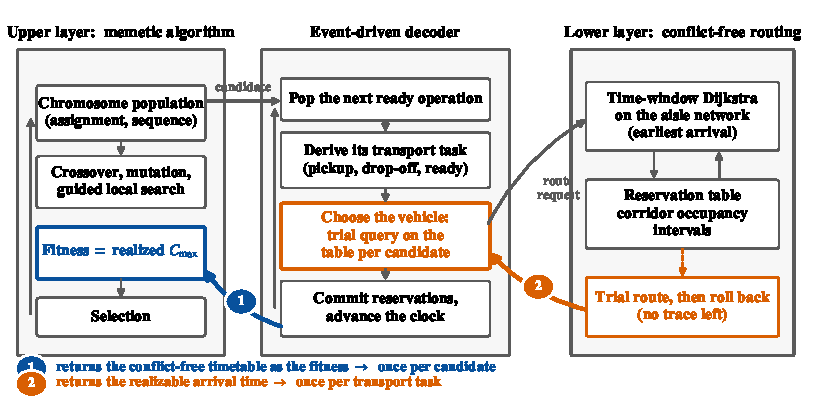
\includegraphics[width=0.8\textwidth]{fig/fig_framework.pdf}
\caption{The closed-loop bilevel framework: memetic search (upper), event-driven decoder (middle), and time-window reservation routing (lower).
Path~1 (blue) returns the conflict-free timetable as fitness, once per candidate; path~2 (orange) runs a two-leg trial query before each vehicle choice, once per transport task, without writing the final timetable.
The ladder of Section~\ref{sec:Chapter_V} is arranged by which paths are open.}
\Description{Schematic of the framework: an upper memetic search layer, an
event-driven decoder, and a lower reservation-based routing layer, with two
colour-coded feedback paths entering the upper layer at different places.}
\label{fig:framework}
\end{figure*}

\subsection{Lower level: time-window reservation and conflict-free routing}
\label{sec:router}

The reservation table maps each corridor, the only contended resource (A6), to a time-ordered list of half-open occupancy intervals $[t,\,t+\tau_e)$ labelled by vehicle and task.
It supports four operations: earliest feasible entry no earlier than a given instant; write; revoke a task; and checkpoint and rollback around a trial query.
Nodes take zero time and waits occur at berths, so nodes are not reserved, and both the conflict-free path planner (hereafter, the router) and an independent checker inspect only corridor occupancy.

The router is a time-window Dijkstra search (Algorithm~\ref{alg:route}) whose label $(u,t)$, with cost $t$, means standing at the berth of $u$ at time $t$.
For each corridor leaving $u$ the table returns the earliest feasible entry $t'\ge t$, so the berth wait $t'-t$ of Eq.~\eqref{eq:walk} is produced by the search itself.
Written paths are not revoked within a decode, so vehicles are planned in task-generation order and a later-planned vehicle yields to an earlier one.

\begin{lem}[One earliest-arrival label per node suffices]
\label{lem:label}
Keeping only the earliest-arrival label at each node is sufficient to obtain a path that reaches the destination earliest under the current reservation table.
\end{lem}

\begin{proof}
Ample berths occupy no corridor (A6), so a vehicle at $u$ since $t$ can wait until any $t'>t$ and take every continuation open to one arriving at $t'$; an earlier label is never worse.
Later queries see no more free slots, so $t\mapsto R.\textsc{EarliestEntry}(e,t,\tau_e)+\tau_e$ is non-decreasing; labels leave the queue in increasing time, so the first extraction of the destination is the earliest arrival.
\end{proof}

Ordinary Dijkstra therefore suffices, without the per-interval labelling of Safe Interval Path Planning (SIPP)~\cite{kasaura2022sipp}; a second criterion such as a surcharge would require a multi-label search (Section~\ref{sec:interface}).

\begin{algorithm}[t]
  \caption{\textsc{Route}: conflict-free planning of a single leg}
  \label{alg:route}
  \footnotesize
  \begin{algorithmic}[1]
  \Require $s$, $g$, departure $t_0$, table $R$, flag \textit{commit}
  \State push $(s,t_0)$ onto a queue keyed by (time, node id)
  \While{the queue is nonempty}
    \State pop the least label $(u,t)$
    \If{$u=g$} \State backtrack occupancies; write them if \textit{commit}; \Return $t$ \EndIf
    \ForAll{corridors $e=(u,v)$}
      \State $t_{\text{in}} \gets R.\textsc{EarliestEntry}(e,t,\tau_e)$; update $(v,\,t_{\text{in}}+\tau_e)$ if strictly earlier
    \EndFor
  \EndWhile
  \State \Return failure \Comment{unreachable; see text}
  \end{algorithmic}
\end{algorithm}

A path always exists because reservations are finite and $G$ is strongly connected: at worst the vehicle waits until every occupancy has ended, then takes an unimpeded shortest path.
With $W$ the mean number of intervals per corridor, a call costs $O\bigl(|E|\,(W^{2}+\log|V|)\bigr)$ ($O(W)$ candidate entries per corridor, each tested in $O(W)$); a logarithmic earliest-entry query would give $O\bigl(|E|(\log W+\log|V|)\bigr)$, but we use the linear scan.
On an empty table the search yields $t^{*}$, used for open-loop estimates, the reassignment proximity term, the two-stage baseline, and the pruning bound (Section~\ref{sec:speedup}).

\subsection{Upper level: encoding and event-driven decoding}
\label{sec:upper}

An individual has two segments: a machine-assignment vector whose $k$-th entry is the arm chosen from $\Omega_{ji}$ for the $k$-th of the $N$ operations, and an operation sequence in which job $j$ appears $n_j$ times (plus once for its dummy when $\delta_{\mathrm{ret}}=1$), its $x$-th appearance standing for $O_{jx}$; operations sharing an arm are ordered by the sequence.
Vehicles are chosen at decode time (Section~\ref{sec:dispatch}), since a third segment would enlarge the search space and lose guaranteed decodability.

The decoder (Algorithm~\ref{alg:decode}) implements the evaluation path.
Sweeping the sequence, it generates a task of Eq.~\eqref{eq:tasks} whenever an operation's arm differs from the job's location, chooses a vehicle, and plans the empty and loaded legs against the live table, joined by Eq.~\eqref{eq:load}.
The operation starts by Eq.~\eqref{eq:bind}, and the recorded \texttt{bind} field (waiting for the workpiece or for the arm) is authoritative for later tracing of postponed starts.

\begin{algorithm}[t]
\caption{\textsc{Decode}: fitness from a complete conflict-free simulation}
\label{alg:decode}
\footnotesize
\begin{algorithmic}[1]
\Require assignment $x$, operation sequence
\State $F_m,\mathrm{ready}_j,\mathrm{avail}_k\gets 0$; $\mathrm{pos}_j,\mathrm{loc}_k\gets v_0$; clear $R$
\ForAll{$O_{ji}$ in sequence order (dummies included)}
  \State $d\gets \mathrm{loc}(m)$ for the arm $m$ of $O_{ji}$ under $x$
  \If{$\mathrm{pos}_j=d$} \State $A_{ji}\gets \mathrm{ready}_j$
  \Else
     \State choose vehicle $k$ (Section~\ref{sec:dispatch}); $a^{\mathrm{E}}\gets\textsc{Route}(\mathrm{loc}_k,\mathrm{pos}_j,\mathrm{avail}_k,R,\text{true})$
     \State $A_{ji}\gets\textsc{Route}(\mathrm{pos}_j,d,\max(a^{\mathrm{E}},\mathrm{ready}_j),R,\text{true})$; $\mathrm{loc}_k,\mathrm{avail}_k\gets d,A_{ji}$
     \State accumulate yielding time by corridor
  \EndIf
  \State $\texttt{bind}\gets\texttt{machine}$ if $F_m>A_{ji}$, else $\texttt{arrive}$
  \State $S_{ji}\gets\max(A_{ji},F_m)$; $C_{ji}\gets S_{ji}+p_{ji}$; $F_m,\mathrm{ready}_j\gets C_{ji}$; $\mathrm{pos}_j\gets d$
\EndFor
\State \Return $\max_{j,i} C_{ji}$, timetable, yield statistics
\end{algorithmic}
\end{algorithm}

Decoding is deterministic: reservations are written in task-generation order, the routing queue breaks ties by node id and updates a label only on a strictly earlier arrival, and dispatching scans vehicles by increasing id and keeps the first strictly better one.
A chromosome thus maps to a unique timetable, on which the seed-paired, equal-budget comparisons of Section~\ref{sec:Chapter_V} depend.

\begin{prop}[Every chromosome is decodable]
  \label{prop:decodable}
  For any machine assignment and any operation sequence, Algorithm~\ref{alg:decode} terminates and returns a conflict-free, deadlock-free timetable of finite makespan. The search therefore need not invoke a repair operator.
\end{prop}

\begin{proof}
The sequence is a topological order of each job's chain, so $\mathrm{ready}_j$ is known when read, and ample buffers (A4) let Eq.~\eqref{eq:bind} give a finite start once the job has arrived.
Each \textsc{Route} call terminates by the existence argument after Algorithm~\ref{alg:route} and occupies only free slots, so Eq.~\eqref{eq:excl} holds by construction.
Deadlock cannot occur: the corridor is the only contended resource (A6), waits occupy only ample berths, and every written occupancy ends at a finite time, so no circular wait arises.
The sweep runs $N+n\delta_{\mathrm{ret}}$ times, each scheduling finitely many events at finite times.
\end{proof}

\subsection{Reservation-table-aware dispatching}
\label{sec:dispatch}

The open-loop rule scores each vehicle by its unimpeded-shortest-path delivery estimate,
\begin{equation}
\label{eq:rule}
\mathrm{score}(k)=\max\bigl(\mathrm{avail}_k+t^{*}(\mathrm{loc}_k,\text{pickup}),\,
\mathrm{ready}_j\bigr)+t^{*}(\text{pickup},\text{destination}),
\end{equation}
the idle-first dispatching of Li et al.~\cite{li2026framework} and a typical single-attribute rule in multi-AGV dispatching~\cite{lu2022agv}; ignoring the reservation table, it may pick a nearby vehicle whose corridors are already occupied.
The closed-loop default, reservation-table-aware dispatching, runs a trial query per candidate vehicle: the empty leg is planned and temporarily written (otherwise both legs could share a corridor--time slot and the result would be too early), the loaded leg is planned against that state, the earliest feasible delivery is recorded, and the table is rolled back.
The vehicle with the earliest feasible delivery is selected; since vehicles are identical (A5) and differ only in location and corridor occupancy, contention on the table can directly determine the choice.
The cost is up to $2N_A$ instead of $2$ routing calls per task, about \CostMultBefore{} times the evaluation cost of rule-based dispatching; unless reduced (Section~\ref{sec:speedup}), this overhead offsets the makespan gain under an equal wall-clock budget, so Section~\ref{sec:Chapter_V} compares the two rules only under the same wall-clock limit.

\subsection{Low overhead: admissible lower-bound pruning and winner-path reuse}
\label{sec:speedup}

At equal generations reservation-table-aware dispatching beats rule-based dispatching by \GainProbeSameGen{}, but at equal wall-clock time its \CostMultBefore{}-fold evaluation cost leaves a net effect close to zero; the two speed-ups below reduce this multiple without changing any selection.

\paragraph{Admissible lower-bound pruning.}
Yielding can only delay routing, never beat the shortest path that ignores contention, so the open-loop estimate of Eq.~\eqref{eq:rule} is an admissible lower bound on the realized delivery time:
\begin{equation}
\label{eq:lb_dispatch}
\mathrm{lb}(k)=\max\bigl(\mathrm{avail}_k+t^{*}(\mathrm{loc}_k,\text{pickup}),\,
\mathrm{ready}_j\bigr)+t^{*}(\text{pickup},\text{destination})\ \le\ \mathrm{est}(k),
\end{equation}
where $\mathrm{est}(k)$ is the earliest feasible delivery from a complete two-leg trial query for vehicle $k$.
A vehicle whose bound is no earlier than the best trial-query delivery so far needs no routing call.

\paragraph{Winner-path reuse.}
Rollback discards the winner's two legs, which the decoder would replan on the same restored table; as routing is deterministic, the cached trial-query paths are written directly, saving two calls.

\begin{prop}[The two speed-ups do not change the selected vehicle or the timetable]
  \label{prop:speedup_equiv}
  In the implementation, vehicles are queried in increasing id order, and the selected vehicle is replaced only when some vehicle's feasible delivery is strictly earlier than the current best.
  Under this rule, after the pruning of Eq.~\eqref{eq:lb_dispatch} and winner-path reuse are added, the selected vehicle, the occupancies written to the reservation table, and the final timetable are the same as when a complete two-leg trial query is run for every vehicle.
\end{prop}

\begin{proof}
If $\mathrm{lb}(k)\ge\mathrm{est}^{\ast}$, the current best, then $\mathrm{est}(k)\ge\mathrm{lb}(k)\ge\mathrm{est}^{\ast}$ by Eq.~\eqref{eq:lb_dispatch}, so $k$ is not strictly earlier and would not be selected anyway; pruned vehicles write nothing to the table, which is restored after each trial query, so later queries are unaffected.
The winner's legs were computed against the very table state the decoder writes into after restoration, and routing is deterministic, so cached and replanned paths give identical occupancies.
\end{proof}

Jointly, measured as one on/off switch (Table~\ref{tab:prune}) and not attributed to pruning or reuse separately, the speed-ups give a \SpeedupProbe{}-fold speed-up, cut routing calls by \RouteCallCut{}, and reduce the cost multiple from \CostMultBefore{} to \CostMultAfter{}.
Trial-query cost grows roughly linearly with $N_A$, and pruning weakens as the fleet grows yet still cuts \RouteCallCutLo{} of the calls on the largest fleet tested; the gain may thus vanish beyond some fleet size, which the present number of seeds is not sufficient to determine (Section~\ref{sec:whichcongestion}).

\subsection{Two further inter-layer interfaces: surcharges and yield records}
\label{sec:interface}\label{sec:ls}

Both paths read realized durations, i.e.\ traversal times after conflict-free routing, for every candidate, whereas schedule-then-route methods obtain them once, after the assignment is fixed.
Realized durations do not reveal which decision caused a wait, so we implement two richer interfaces and compare them under an equal wall-clock budget (Section~\ref{sec:pricing}).

A \emph{surcharge} $\pi(e,b)$, by analogy with shadow prices in Lagrangian relaxation and column generation, is added to arrival time by a vehicle occupying corridor $e$ in slot $b$: routing minimizes arrival time $+\,\theta\cdot$ the surcharges traversed (the surcharge coefficient $\theta\ge0$ is the only tunable parameter), and reassignment likewise pays for its traversals.
$\pi$ is estimated by perturbing one slot's capacity and re-solving, or by a low-cost approximation refreshed each generation.
While fitness comes from a complete conflict-free decode, such a cost adds no information: contention wait already enters arrival time, makespan (Eq.~\eqref{eq:bind}) and fitness, so the surcharge counts it twice, and blocking of later tasks already shows in the decoded makespan; we verify this inference on this one interface only.
By Lemma~\ref{lem:label}, the second criterion also forces a multi-label Pareto search, raising evaluation cost whether or not the surcharge is non-zero.

A \emph{yield record} instead returns structure: the triple (corridor, time slot, preceding occupying transport) that routing knows at each yield.
It enters no objective, so no delay is double-counted; it only shapes the neighbourhood of yield-record-guided local search, applied with the same setting to the top-ranked individuals of each generation in all four main-batch configurations.
The search backtracks from the makespan-determining event along a critical chain that includes transport legs, since a wait for the workpiece may stem from an upstream operation, a missing vehicle, or contention; links are labelled as in Table~\ref{tab:attrib}, a yield on a loaded leg counting as \texttt{corridor} and an empty leg classified by whether yielding exceeds half its duration.
For each of at most $L=5$ real operations on the chain, reassignment yields one neighbour by moving it from arm $m$ to the arm $m'\in\Omega_{ji}\setminus\{m\}$ minimizing
\begin{equation}
\label{eq:reassign}
\mathrm{score}(m')=t^{*}\bigl(d_{j,i-1},\mathrm{loc}(m')\bigr)+t^{P}_{jim'},
\end{equation}
trading a longer processing time for a shorter path with better traffic (cumulative yield, a fleet- and horizon-wide total, is not commensurable and is omitted).
Staggering advances the blocked operation or postpones the preceding occupier on the longest \texttt{corridor} link by swapping adjacent appearances of different jobs, preserving decodability (Proposition~\ref{prop:decodable}).
The first improvement among these at most $L+2=7$ neighbours is accepted, for at most three rounds with the chain recomputed each round; the same tracing reads the case study (Section~\ref{sec:casestudy}).

\begin{table}[t]
\caption{Critical-chain link labels and remedies. Only \texttt{corridor} names a corridor, time slot, and preceding transport.}
\label{tab:attrib}
\footnotesize
\begin{tabular}{@{}llp{2.3cm}@{}}
\toprule
Label & Criterion & Remedy \\
\midrule
\texttt{operation} & a real operation occupies its arm & --- \\
\texttt{machine} & waiting for the arm & resequence \\
\texttt{upstream} & vehicle first, material not ready & recurse to $O_{j,i-1}$ \\
\texttt{vehicle} & material ready, vehicle late, little yielding & change vehicle \\
\texttt{corridor} & yield on a given corridor and slot & reassignment or staggering \\
\bottomrule
\end{tabular}
\end{table}

\subsection{Outer genetic algorithm, complexity and cost}

The outer layer is a conventional genetic algorithm: a random initial population plus a fastest-arm and a greedy load-balancing individual; tournament selection with a small elite; precedence-preserving order crossover on the sequence, uniform crossover on the assignment; and swap or reassignment mutation (hyperparameters in Section~\ref{sec:impl}).

One evaluation processes $N+n\delta_{\mathrm{ret}}$ events with at most $2N_A$ routing calls per transport under closed-loop dispatching, so an individual costs $O\bigl((N+n)\,N_A\,|E|\,(W^{2}+\log|V|)\bigr)$; open-loop selection drops the factor $N_A$.
The speed-ups leave this bound and every selection unchanged (Proposition~\ref{prop:speedup_equiv}) but cut routing calls by \RouteCallCut{} (\RouteCallCutLo{} to \RouteCallCutHi{} across instances), in effect shrinking $N_A$; local search adds at most $3(L+2)=21$ decodes per selected individual.
On the ladder batch one evaluation takes \MsOpen{}\,ms open-loop, \MsLoopRule{}\,ms with rule-based dispatching, and \MsLoopProbe{}\,ms full closed-loop (about $37$ times open-loop); in an earlier scan the surcharge raised it from \MsPricedRef{}\,ms to \MsPriced{}\,ms (about $4.8$ times), so costs span about two orders of magnitude, although the two batches' timings are not directly comparable.
A costlier evaluation buys fewer evaluations, so whether an interface pays off must be measured, and Section~\ref{sec:Chapter_V} aligns wall-clock time rather than generations.

These results guarantee correctness, not solution quality: Proposition~\ref{prop:decodable}, Lemma~\ref{lem:label}, and Proposition~\ref{prop:speedup_equiv} ensure that every candidate is feasible, that its evaluation matches the conflict model of Section~\ref{sec:Chapter_III}, and that the speed-ups change no selection, and deterministic decoding makes the procedure reproducible.
As with most metaheuristics, solution quality has no theoretical bound and is evaluated experimentally in the next section.
